\documentclass{article}

\usepackage[left=2cm,right=2cm,top=2cm,bottom=2cm]{geometry} 

\usepackage[utf8]{inputenc}   % otra alternativa para los caracteres acentuados y la "ñ"
\usepackage[           spanish % para poder usar el español
                      ,es-tabla % para los captions de las tablas
                       ]{babel}   
\decimalpoint %para usar el punto decimal en vez de coma para los números con decimales

%\usepackage{beton}
%\usepackage[T1]{fontenc}

\usepackage{parskip}
\usepackage{xcolor}

\usepackage{caption}

\usepackage{enumerate} % paquete para poder personalizar fácilmente la apariencia de las listas enumerativas

\usepackage{graphicx} % figuras
\usepackage{subfigure} % subfiguras

\usepackage{amsfonts}
\usepackage{amsmath}

\definecolor{gris}{RGB}{220,220,220}
	
\usepackage{float} % para controlar la situación de los entornos flotantes

\restylefloat{figure}
\restylefloat{table} 
\setlength{\parindent}{0mm}


\usepackage[bookmarks=true,
            bookmarksnumbered=false, % true means bookmarks in 
                                     % left window are numbered
            bookmarksopen=false,     % true means only level 1
                                     % are displayed.
            colorlinks=true,
            allcolors=blue,
            urlcolor=blue]{hyperref}
\definecolor{webblue}{rgb}{0, 0, 0.5}  % less intense blue


\title{\Huge Inteligencia de Negocio: Práctica 1 \\ Resolución de problemas
  de clasificación y análisis experimental\vspace{10mm}}

\author{\huge David Cabezas Berrido \vspace{10mm} \\ 
  \huge Grupo 2: Viernes \vspace{10mm} \\ \huge dxabezas@correo.ugr.es \vspace{10mm}}

\begin{document}
\maketitle
\newpage
\tableofcontents
\newpage

\section{Introducción}

En esta primera práctica abordaremos el problema de decidir si un
tumor en una mamografía es benigno o maligno, por lo que deducimos que
se trata de un problema de clasificación binaria (dos clases: benigno
y maligno). Disponemos para ello de datos de 961 pacientes, para cada
uno de ellos se han medido 6 atributos entre cualitativos y
cuantitativos.

Sobre este problema real, pondremos a prueba los distintos algoritmos
estudiados en teoría y las herramientas de prácticas. Trataremos de
mejorar los resultados mediante el procesado de los datos y
probando distintos hiperparámetros en los algoritmos. Finalmente,
compararemos los algoritmos entre sí y discutiremos cuál es el más
adecuado para el problema.

Para la experimentación usaremos validación cruzada de 5
particiones. La matriz de confusión se calculará como la suma de las
matrices de confusión de cada partición, de esta forma la matriz
resultante tendrá en cuenta cada instancia una sola vez. Como usamos
validación cruzada, nos ahorramos tener que separar un conjunto de
test para pruebas y aprovechamos cada instancia tanto para
entrenamiento como para evaluación.

Para esta tarea, utilizaremos las herramientas \textit{pandas}, para
tratamiento y visualización de datos; y \textit{sklearn} para el
preprocesado y la creación de los modelos.

Empezamos analizando el dataset. Como ya hemos comentado, consta de
961 instancias y cuenta con 6 atributos: 

\begin{enumerate}
\item Código \href{https://es.wikipedia.org/wiki/BI-RADS}{BI-RADS}: se
  trata de un número entero entre 0 y 6 (ambos incluidos) asignado por
  un radiólogo tras interpretar la mamografía. Un mayor valor
  significa una mayor probabilidad de malignidad, a excepción del
  valor 0, que indica que la información de la radiografía es
  insuficiente. Tendremos que tener esto en cuenta, ya que puede
  ``confundir'' a algunos algoritmos como el KNN, que interpretaría
  que un código 0 está más próximo a un código 1 que a un código 4, lo
  cual no tiene sentido a priori (sin atender a más características).

\item Edad del paciente: entero positivo.
\item Forma del tumor: nominal, 4 posibles formas distintas (R, O, L,
  I) y N para indicar que la forma no está definida.
\item Margen de la masa: nominal, 5 posibles valores (del 1 al 5).
\item Densidad de la masa: entero entre 1 y 4 (ambos inclusive), un
  menor valor indica mayor densidad.
\item Severidad: variable objetivo a predecir, benigno o maligno. 
\end{enumerate}

Hay algunos datos perdidos en el dataset: \vspace{-5mm}
\begin{table}[H]
  \centering
  \begin{tabular}{c|c}
    BI-RADS     & 2 \\
    Age         & 5 \\
    Shape       & 0 \\
    Margin      & 48 \\
    Density     & 76 \\
    Severity    & 0
  \end{tabular}
\end{table}
\vspace{-8mm} En principio, no hay los suficientes datos perdidos como
para dejar de considerar alguna variable, pero durante el procesado de
datos discutiremos si eliminar alguna o cómo imputar los datos
perdidos.

De los 961 instancias, 445 pertenecen a la clase maligno (46.3\%) y
516 a benigno (53.7\%). Las clases están bastante balanceadas, lo que
en genral convierte a la accuracy en una métrica bastante adecuada y
fácil de interpretar (proporción de ejemplos bien clasificados) para
la bondad de los algoritmos de clasificación. Sin embargo, en este
problema concreto, parece mucho más grave un falso negativo
(predecimos benigno y enviamos a un paciente a casa que debería
empezar a tratarse) que un falso positivo (predecimos maligno y el
paciente irá a análisis posteriores donde probablemente se percaten
del error); por lo que puede ser interesante considerar otras métricas
de evaluación.

En concreto, las métricas F1-score y G-measure, medias armónica y
geométrica respectivamente de PPV (proporción de correctas entre las
predicciones positivas) y TPR (proporción de correctas entre los
ejemplos positivos), penalizan más los errores a la hora de clasificar
instancias positias (malignas). Esto las hace más adecuadas para el
problema, por lo que les daremos mayor importancia a la hora de
discutir cuando un algoritmo, configuración o procesamiento es mejor
que otro.

Los algoritmos que pondremosm a prueba son: Árbol de Decisión,
Naive-Bayes, SVM, Random Forest, KNN y Redes Neuronales. Los
introduciremos en la sección \ref{resultados}, excepto los que
configuremos previamente, que los explicaremos en \ref{configuracion}.

\section{Procesado de datos}

Presentamos distintas técnicas de preprocesado de los
datos. Discutiremos, para cada una de ellas, su efecto (bueno o malo)
sobre los resultados de los algoritmos. Para comparar la bondad de los
procesamientos, ejecutaremos todos los algoritmos a comparar con
parámetros por defecto sobre esos datos y atenderemos a los score
medio y máximo conseguidos entre los modelos (ignorando el
\texttt{DummyClassifier}).

En todas ellas debemos usar \texttt{LabelEncoder} (de
\textit{sklearn}), porque los algoritmos de esta librería necesitan
trabajar con datos numéricos.

\subsection{Preprocesado 1: Eliminación de valores perdidos}

La mayoría de los algoritmos no aceptan como entrada datos con valores
perdidos, esto se podría solucionar asignando un valor fijo a estos
valores que represente valor perdido, o simplemente podemos eliminar
los valores perdidos con el método \texttt{dropna} del objeto
\texttt{DataFrame} de \textit{pandas}. Este es un preprocesado muy
básico, prácticamente el justo para que funcionen los algoritmos, y
debería ser superado a medida que experimentemos con procesamientos
más avanzados.

Hay que tener en cuenta que el valor 0 en el código BI-RADS significa
radiografía insuficiente, y el valor N en la forma significa que la
forma no está definida. Así que consideraremos estos valores como
perdidos.

Ejecutamos los algoritmos sobre estos datos y obtenemos los siguientes
resultados:

\begin{table}[H]
\centering
\caption{Eliminación de instancias con valores perdidos}
\label{tab:dropna}
\begin{tabular}{|lrrrrrrrrrr|}
\hline
 & TP & TN & FP & FN & Acc & TPR & FPR & AUC & F1-score & G-measure\\ \hline
Dummy & 400 & 0 & 425 & 0 & 0.4848 & 1.0 & 1.0 & 0.5 & 0.6531 & 0.6963\\
DecisionTree & 288 & 341 & 84 & 112 & 0.7624 & 0.72 & 0.1976 & 0.7612 & 0.7461 & 0.7466\\
GaussianNB & 341 & 340 & 85 & 59 & 0.8255 & 0.8525 & 0.2 & 0.8263 & 0.8257 & 0.8261\\
SupportVectorM & 331 & 314 & 111 & 69 & 0.7818 & 0.8275 & 0.2612 & 0.7832 & 0.7862 & 0.7872\\
RandomForest & 312 & 345 & 80 & 88 & 0.7964 & 0.78 & 0.1882 & 0.7959 & 0.7879 & 0.7879\\
KNN & 330 & 333 & 92 & 70 & 0.8036 & 0.825 & 0.2165 & 0.8043 & 0.8029 & 0.8032\\
NeuralNetwork & 337 & 332 & 93 & 63 & 0.8109 & 0.8425 & 0.2188 & 0.8118 & 0.812 & 0.8126\\ \hline
Máximo & 341 & 345 & 111 & 112 & 0.8255 & 0.8525 & 0.2612 & 0.8263 & 0.8257 & 0.8261\\
Media & 323.2 & 334.2 & 90.8 & 76.8 & 0.7968 & 0.8079 & 0.2137 & 0.7971 & 0.7935 & 0.7939\\
\hline
\end{tabular}
\end{table}

\subsection{Preprocesado 2: Imputación de valores perdidos}

Rellenamos los valores perdidos con algún valor para no tener que
eliminar una instancia y poder aprovechar así el resto de datos de la
instancia (los no perdidos). Para las variables numéricas,
discutiremos 2 formas de hacer esto: la media y la mediana de la
columna. En cambio las nominales las imputaremos usando la moda.

Para esta tarea utilizamos el objeto SimpleImputer de
\textit{sklearn}, debemos indicarle la estrategia que queremos que
utilice. Como hemos comentado: probaremos \texttt{'mean'} y
\texttt{'median'} para las varaiables numéricas y
\texttt{'most\_frequent'} para las nominales. Antes de continuar, nos
quedaremos con la estrategia para las variables numéricas que consiga
los mejores resultados.

\begin{table}[H]
\centering
\caption{Imputando valores perdidos numéricos con la media}
\label{tab:impute-mean}
\begin{tabular}{|lrrrrrrrrrr|}
\hline
 & TP & TN & FP & FN & Acc & TPR & FPR & AUC & F1-score & G-measure\\ \hline
Dummy & 445 & 0 & 516 & 0 & 0.4631 & 1.0 & 1.0 & 0.5 & 0.633 & 0.6805\\
DecisionTree & 316 & 420 & 96 & 129 & 0.7659 & 0.7101 & 0.186 & 0.762 & 0.7375 & 0.738\\
GaussianNB & 374 & 413 & 103 & 71 & 0.8189 & 0.8404 & 0.1996 & 0.8204 & 0.8113 & 0.8118\\
SupportVectorM & 360 & 393 & 123 & 85 & 0.7836 & 0.809 & 0.2384 & 0.7853 & 0.7759 & 0.7765\\
RandomForest & 338 & 422 & 94 & 107 & 0.7908 & 0.7596 & 0.1822 & 0.7887 & 0.7708 & 0.7709\\
KNN & 341 & 411 & 105 & 104 & 0.7825 & 0.7663 & 0.2035 & 0.7814 & 0.7654 & 0.7654\\
NeuralNetwork & 365 & 410 & 106 & 80 & 0.8065 & 0.8202 & 0.2054 & 0.8074 & 0.7969 & 0.7973\\ \hline
Máximo & 374 & 422 & 123 & 129 & 0.8189 & 0.8404 & 0.2384 & 0.8204 & 0.8113 & 0.8118\\
Media & 349 & 411.5 & 104.5 & 96 & 0.7914 & 0.7843 & 0.2025 & 0.7909 & 0.7763 & 0.7766\\
\hline
\end{tabular}
\end{table}

\begin{table}[H]
\centering
\caption{Imputando valores perdidos numéricos con la mediana}
\label{tab:impute-median}
\begin{tabular}{|lrrrrrrrrrr|}
\hline
 & TP & TN & FP & FN & Acc & TPR & FPR & AUC & F1-score & G-measure\\ \hline
Dummy & 445 & 0 & 516 & 0 & 0.4631 & 1.0 & 1.0 & 0.5 & 0.633 & 0.6805\\
DecisionTree & 318 & 420 & 96 & 127 & 0.768 & 0.7146 & 0.186 & 0.7643 & 0.7404 & 0.7409\\
GaussianNB & 374 & 413 & 103 & 71 & 0.8189 & 0.8404 & 0.1996 & 0.8204 & 0.8113 & 0.8118\\
SupportVectorM & 360 & 393 & 123 & 85 & 0.7836 & 0.809 & 0.2384 & 0.7853 & 0.7759 & 0.7765\\
RandomForest & 335 & 420 & 96 & 110 & 0.7856 & 0.7528 & 0.186 & 0.7834 & 0.7648 & 0.7649\\
KNN & 346 & 414 & 102 & 99 & 0.7908 & 0.7775 & 0.1977 & 0.7899 & 0.7749 & 0.7749\\
NeuralNetwork & 366 & 410 & 106 & 79 & 0.8075 & 0.8225 & 0.2054 & 0.8085 & 0.7983 & 0.7986\\ \hline
Máximo & 374 & 420 & 123 & 127 & 0.8189 & 0.8404 & 0.2384 & 0.8204 & 0.8113 & 0.8118\\
Media & 349.8 & 411.7 & 104.3 & 95.2 & 0.7924 & 0.7861 & 0.2022 & 0.792 & 0.7776 & 0.7779\\
\hline
\end{tabular}
\end{table}

Atendiendo al máximo y a la media de los scores de los algoritmos,
observamos que con este preprocesado decrecen levemente las métricas
Accuracy y AUC (Area Under Curve), que miden la eficiencia general de
los modelos. Lo misimo le ocurre a las métricas F1-score y G-measure,
que son las que se ajustan más a la naturaleza del problema, ya que
penalizan más los falsos positivos. Esto ocurre para las dos
estrategias. Aunque la imputación de valores numéricos por la mediana
ha resultado ligeramente mejor que usando la media, ambas han
empeorado el desempeño de los algoritmos. Por esto decidimos abandonar
la idea de imputar valores y mantenemos las instancias con valores
perdidos eliminadas.

\subsection{Preprocesado 3: Eliminación de características innecesarias}

Estudiaremos si todas las características son útiles a la hora de
predecir. En primer lugar, obtenemos la desviación típica de cada una:

\begin{table}[H]
  \centering
  \begin{tabular}{cccc}
    BI-RADS &  Age & Margin & Density \\ \hline
	0.635706 & 14.480131 & 1.566546 & 0.380444
  \end{tabular}
\end{table}
Observamos una baja varianza en BI-RADS y en Density, usamos
\texttt{Counter} para ver su distribución y observamos que de las 825
instancias sin valores perdidos, hay 468 con el valor 4 para el código
BI-RADS y 317 con el valor 5. Decidimos mantenerla, ya que puede
seguir teniendo interés, aun así, optamos por colapsar el resto de
valores en 4 (los valores 2 y 3) y 5 (valor 6), ya que hay muy pocas
instancias con estos valores (40 en total). 

En el caso de Density, 750 instancias tienen el valor 3, por lo que su
distribución es prácticamente degenerada en 3. Así que decidimos
eliminar esta variable.

Estas dos acciones suponen obviamente una pérdida de información, pero
ayuda a reducir la complejidad de los modelos y los hace más
fácilmente interpretables (la característica se convierte en binaria),
de modo que mantendremos esta decisión siempre que no suponga un
descenso notable en el desempeño de los algoritmos.

No nos muestra la desviación de Shape al no ser numérica, pero
obtenemos igualmente su distribución con \texttt{Counter} y observamos
que está lejos de ser degenerada, así que la mantenemos.

Con el método \texttt{corr} de \texttt{pandas.DataFrame}, obtenemos la
matriz de correlación entre las características. Si encontrásemos dos
atributos altamente correlados, nos plantearíamos si quedarnos con
sólo uno de ellos.

\begin{figure}[H]
  \centering
  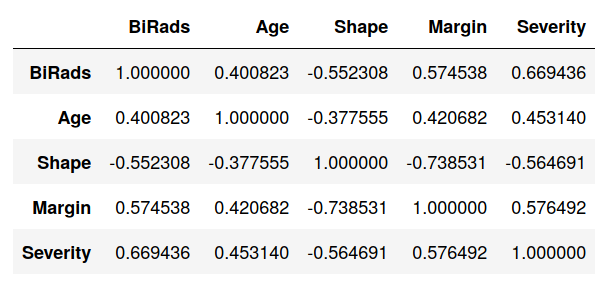
\includegraphics[width=100mm]{figures/corr}
  \caption{Matriz de correlación entre los atributos}
  \label{fig:corr}
\end{figure}

No encontramos ningun par de variables con una correlación alta entre
ellas, el máximo es -0.7385 entre Shape y Margin. De modo que
mantenemos el resto de características.

Los resultados obtenidos son:

\begin{table}[H]
\centering
\caption{Simplificando el conjunto de atributos}
\label{tab:features}
\begin{tabular}{|lrrrrrrrrrr|}
\hline
 & TP & TN & FP & FN & Acc & TPR & FPR & AUC & F1-score & G-measure\\ \hline
Dummy & 400 & 0 & 425 & 0 & 0.4848 & 1.0 & 1.0 & 0.5 & 0.6531 & 0.6963\\
DecisionTree & 293 & 349 & 76 & 107 & 0.7782 & 0.7325 & 0.1788 & 0.7768 & 0.762 & 0.7626\\
GaussianNB & 346 & 347 & 78 & 54 & 0.84 & 0.865 & 0.1835 & 0.8407 & 0.8398 & 0.8402\\
SupportVectorM & 330 & 310 & 115 & 70 & 0.7758 & 0.825 & 0.2706 & 0.7772 & 0.7811 & 0.7822\\
RandomForest & 313 & 345 & 80 & 87 & 0.7976 & 0.7825 & 0.1882 & 0.7971 & 0.7894 & 0.7894\\
KNN & 328 & 335 & 90 & 72 & 0.8036 & 0.82 & 0.2118 & 0.8041 & 0.802 & 0.8022\\
NeuralNetwork & 323 & 338 & 87 & 77 & 0.8012 & 0.8075 & 0.2047 & 0.8014 & 0.7975 & 0.7976\\ \hline
Máximo & 346 & 349 & 115 & 107 & 0.84 & 0.865 & 0.2706 & 0.8407 & 0.8398 & 0.8402\\
Media & 322.2 & 337.3 & 87.7 & 77.8 & 0.7994 & 0.8054 & 0.2063 & 0.7996 & 0.7953 & 0.7957\\
\hline
\end{tabular}
\end{table}

Al comparar los resultados de los algoritmos sobre este procesamiento
con los mejores resultados obtenidos hasta el momento (eliminación de
valores perdidos, Tabla \ref{tab:dropna}), apreciamos una leve mejora
en las métricas Accuracy y AUC, por lo que no ha decaído su capacidad
de predicción. También mejoran levemente los scores F1-score y
G-measure, por lo que los modelos siguen siendo apropiados para el
problema. Esto se debe sobre todo al aumento del desempeño de Gaussian
Naive-Bayes, que supone que los atributos son independientes. Al
simplificar el conjunto de atributos es lógico que disminuya el grado
de dependencia entre los mismos y el algoritmo funcione mejor.

No sólo no hemos observado un descenso en el desempeño de los modelos,
sino una pequeña mejora. Así que mantenemos este preprocesamiento.

\subsection{Preprocesado 4: Binarización de características nominales}

Nuestro dataset tiene dos características nominales: Shape y Margin,
que toman 4 y 5 posibles valores respectivamente. Codificar estas
variables utilizando números naturales puede confundir a algunos
algoritmos. Este es el caso de KNN, que podría interpretar que una
instancia con valor 2 en cualquiera de estas características está más
cerca de una con valor 1 ó 3 que de una con valor 4, cuando no es
lógico pensar esto, ya que estos números simplemente codifican
cualidades. Es por ello que binarizamos estas dos variables
introduciendo 9 nuevos atributos binarios (valdrán 0 ó 1), 4 de ellos
indicarán el valor de Shape (1 en la posición correspondiente al valor
y 0 en las demás) y 5 para el valor de Margin. De esa forma, dos
individuos con distintos valores de la característica Shape estarán a
distancia 0 (por lo que a la variable Shape respecta) si tienen el
mismo valor en esta característica y a una distancia constante
positiva (por lo que a la variable Shape respecta) si tienen valor de
Shape diferente; y análogo para Margin. Esto puede mejorar la
eficiencia de algunos algoritmos, especialmente de KNN.

En este caso, el número de características nominales y de valores que
pueden tomar es bajo, así que esta operación es factible. De haber
existido un número más elevado de características nominales o un
número más elevado de posibles valores para las mismas, binarizar
estas características conllevaría un aumento notable del número de
variables, lo que puede provocar dificultades en el aprendizaje de los
modelos si el número de datos no es lo suficientemente grande.

Para esta tarea utilizamos \texttt{OneHotEnconder}, de
\textit{sklearn}. Los resultados obtenidos son:

\begin{table}[H]
\centering
\caption{Binarización de atributos nominales}
\label{tab:binarization}
\begin{tabular}{|lrrrrrrrrrr|}
\hline
 & TP & TN & FP & FN & Acc & TPR & FPR & AUC & F1-score & G-measure\\ \hline
Dummy & 400 & 0 & 425 & 0 & 0.4848 & 1.0 & 1.0 & 0.5 & 0.6531 & 0.6963\\
DecisionTree & 297 & 347 & 78 & 103 & 0.7806 & 0.7425 & 0.1835 & 0.7795 & 0.7665 & 0.7669\\
GaussianNB & 354 & 321 & 104 & 46 & 0.8182 & 0.885 & 0.2447 & 0.8201 & 0.8252 & 0.8271\\
SupportVectorM & 281 & 307 & 118 & 119 & 0.7127 & 0.7025 & 0.2776 & 0.7124 & 0.7034 & 0.7034\\
RandomForest & 319 & 344 & 81 & 81 & 0.8036 & 0.7975 & 0.1906 & 0.8035 & 0.7975 & 0.7975\\
KNN & 332 & 332 & 93 & 68 & 0.8048 & 0.83 & 0.2188 & 0.8056 & 0.8048 & 0.8052\\
NeuralNetwork & 342 & 337 & 88 & 58 & 0.823 & 0.855 & 0.2071 & 0.824 & 0.8241 & 0.8246\\ \hline
Máximo & 354 & 347 & 118 & 119 & 0.823 & 0.885 & 0.2776 & 0.824 & 0.8252 & 0.8271\\
Media & 320.8 & 331.3 & 93.7 & 79.2 & 0.7905 & 0.8021 & 0.2204 & 0.7908 & 0.7869 & 0.7874\\
\hline
\end{tabular}
\end{table}

Comparamos los resultados con los de la Tabla \ref{tab:features}. Las
métricas Acc. y AUC (que miden la eficacia general de los modelos) han
mejorado levemente en la mayoría de modelos, aunque ha decaído el
máximo score, ya que el mejor modelo hasta el momento (Gaussian
Naive-Bayes) ha visto empeorados sus resultados, la media ha decrecido
porque los resultados de SVM han empeorado drásticamente. No
experimentamos una mejora sustancial en KNN como esperábamos, pero sí
en la Red Neuronal, que también puede sufrir de la condición que hemos
comentado antes, y se convierte en el nuevo máximo. Respecto a las
métricas F1-score y G-measure, que reflejan mejor la naturaleza del
problema, ha ocurrido exactamente lo mismo con la excepción de que la
caída de Gaussian Naive-Bayes y el crecimiento de la Red Neuronal no
han sido suficientes para que la red supere a Naive-Bayes en estas
métricas. Esto ocurre porque la Red Neuronal ha mejorado a Naive-Bayes
gracias a una mejor clasificación en las instancias negativas, a las
que las métricas F1-score y G-measure les dan una menor importancia.

Aquí se nos plantea una elección difícil sobre cual sería mejor
procesamiento, podemos mantener el que teníamos y apostar por
Naive-Bayes; o adoptar el nuevo, y disponer de una gama más amplia
pero hasta ahora menos efectiva de algoritmos. Nos decantaremos por
binarizar los atributos nominales, debido al poco interés que se le ha
dado a Naive-Bayes en clase de teoría y la facilidad de interpretación
que poseen los árboles.

\subsection{Preprocesado 5: Reescalado de los datos}

Otro problema de los datos que puede provocar dificultades en el
aprendizaje de los algoritmos es el hecho de que los datos tengan
distinta naturaleza y por tanto distinta escala. Pongaos un ejemplo:
si una variable toma valores de un orden entre 10 y 100 como es la
edad, y otra variable toma valores entre 20000 y 200000 como podrían
ser ingresos anuales en euros. Un algoritmo como KNN o Red Neuronal,
interpretaría que 20 años de diferencia entre dos sujetos equivaldría
a 20 euros al año de diferencia en sus ingresos, lo cual no es lógico
pensar. Es por esto que algunas variables estarían teniendo un papel
más relevante que otras, según su naturaleza. En nuestro caso, la
variable Age estaría cobrando más relevancia que otras.

Para solucionar este problema recurrimos a un reescalado de las
variables, de tal forma que todas tengan media 0 y desviación típica
1. Utilizamos para ello el objeto \texttt{StandardScaler} de
\textit{sklearn}.

\begin{table}[H]
\centering
\caption{Estandarizando los datos}
\label{tab:stdScaler}
\begin{tabular}{|lrrrrrrrrrr|}
\hline
 & TP & TN & FP & FN & Acc & TPR & FPR & AUC & F1-score & G-measure\\ \hline
Dummy & 400 & 0 & 425 & 0 & 0.4848 & 1.0 & 1.0 & 0.5 & 0.6531 & 0.6963\\
DecisionTree & 297 & 347 & 78 & 103 & 0.7806 & 0.7425 & 0.1835 & 0.7795 & 0.7665 & 0.7669\\
GaussianNB & 354 & 321 & 104 & 46 & 0.8182 & 0.885 & 0.2447 & 0.8201 & 0.8252 & 0.8271\\
SupportVectorM & 333 & 364 & 61 & 67 & 0.8448 & 0.8325 & 0.1435 & 0.8445 & 0.8388 & 0.8388\\
RandomForest & 320 & 341 & 84 & 80 & 0.8012 & 0.8 & 0.1976 & 0.8012 & 0.796 & 0.796\\
KNN & 324 & 350 & 75 & 76 & 0.817 & 0.81 & 0.1765 & 0.8168 & 0.811 & 0.811\\
NeuralNetwork & 333 & 355 & 70 & 67 & 0.8339 & 0.8325 & 0.1647 & 0.8339 & 0.8294 & 0.8294\\ \hline
Máximo & 354 & 364 & 104 & 103 & 0.8448 & 0.885 & 0.2447 & 0.8445 & 0.8388 & 0.8388\\
Media & 326.8 & 346.3 & 78.7 & 73.2 & 0.816 & 0.8171 & 0.1851 & 0.816 & 0.8111 & 0.8115\\
\hline
\end{tabular}
\end{table}

Comparando con la Tabla \ref{tab:binarization}, en las métricas Acc.,
AUC, F1-score y G-measure apreciamos una gran mejora en todos los
algoritmos salvo los árboles y en Naive-Bayes que acostumbran a tratar
las características individualmente (los árboles en cada nodo trabajan
con una única característica). La mayor mejora se observa en SVM, este
algoritmo se beneficia bastante de la estandarización, y esto nos hace
pensar que su mal desempeño anterior ocurrió porque al binarizar las
características nominales reducimos aun más su escala. Pasamos de
características con valores del 1 al 4 (Shape) ó 5 (Margin), a un
número más elevado de características binarias. Esto supone que exista
más diferencia de escalas con respecto a Age, lo que claramente
observamos que perjudica a SVM.

Tras este análisis comparativo de los preprocesados, llegamos a este
último, que combina las diferentes decisiones que hemos ido tomando
(cada técnica de preprocesamiento se ha aplicado sobre la mejor de las
anteriores). Éste será el procesamiento sobre el que configuremos los
modelos.

\section{Configuración de algoritmos} \label{configuracion}

% Statistical learning
http://faculty.marshall.usc.edu/gareth-james/ISL

\section{Resultados obtenidos} \label{resultados}

Presentamos los distintos modelos y los resultados obtenidos por cada
uno.

\section{Análisis de resultados} \label{sec:analisis}

\subsection{Sobre preprocesado básico}

\subsection{Sobre preprocesado 1 (Imputación de valores perdidos)}

\section{Interpretación de resultados}

\section{Contenido adicional}

\section{Bibliografía/Webgrafía}

http://faculty.marshall.usc.edu/gareth-james/ISL
% TODO BI-RADS
% TODO mamographic: BI-RADS no predictiva
% Yaser

\end{document}
